%%%%%%%%%%%%%%%%%%%%%%%%%%%%
    %%% [INTRODUCAO] %%%
%%%%%%%%%%%%%%%%%%%%%%%%%%%%
\section{Introdução}
    
    Indústrias como a do vidro, do aço e da madeira, entre outras que trabalham com o corte ou a embalagem de materiais, estão constantemente buscando otimizar seus processos produtivos para se manterem competitivas no mercado atual, altamente desafiador e globalizado. Buscar maneiras de reduzir o desperdício de matéria-prima é uma estratégia crucial para essas empresas, visando minimizar os custos de produção e melhorar a eficiência operacional (\cite{Morabito1998}), (\cite{hopper2000two}), (\cite{Morabito2000}), (\cite{Cintra2007}), (\cite{Parreno2021}). Nesse contexto, o problema de corte e empacotamento bidimensional, conhecido como \emph{Strip Packing Problem} (\emph{SPP}) 2D, desempenha um papel fundamental.

    No \emph{SPP-2D}, o objetivo é encontrar a melhor forma de alocar um conjunto de itens em um objeto bidimensional, de modo a minimizar o desperdício de área (\cite{hopper2000two}). A proposta original do problema é determinar a altura mínima do objeto necessário para atender às demandas de corte ou empacotamento dos itens (\cite{Cherri2009}). Essa abordagem está diretamente relacionada aos desafios enfrentados pelas indústrias mencionadas anteriormente. Diversos métodos de resolução foram desenvolvidos para maximizar a utilização da área disponível no objeto, considerando características como a forma dos itens (regulares ou irregulares), a possibilidade de rotação dos itens e o tipo de corte do objeto (guilhotinado ou não-guilhotinado).

    Os métodos propostos para o \emph{SPP} apresentam abordagens diferentes para resolver o problema. Com isso, para poder dizer se um modelo é eficiente ou não, é necessário realizar uma bateria de testes com instâncias já conhecidas na literatura e analisar o desempenho do método, na busca pela melhor configuração dos itens no objeto, considerando o tempo necessário para encontrar uma solução e a diferença entre os resultados já encontrados para o problema.

    Uma abordagem que pode ser considerada para solucionar o problema, otimizando a área aproveitada do objeto, é a redução do perímetro ou a redução da área. Esses modelos, de dimensões abertas, buscam encontrar uma configuração dos itens que minimize o espaço sobressalente no objeto, diferente da abordagem original, que trabalha com a largura fixa e visa minimizar apenas a altura do objeto.

    %%%%%%%%%%%%%%%%%%%%%%%%%%%%%%%%%%%%%%%%%
    %%% Exemplo da rotacao comentada.
    %%% Inserir outro exemplo sem rotacao.
    %%%%%%%%%%%%%%%%%%%%%%%%%%%%%%%%%%%%%%%%%
    \begin{comment}
        Na Figura~\ref{Fig-Exemplos-sem-rotacao} é apresentado um exemplo de aplicação desses três métodos, desconsiderando a rotação dos itens, para uma instância pequena. Nesse exemplo, a dimensão dos itens impede que os modelos encontrem a melhor configuração para o problema. Cada método consegue obter o melhor resultado para sua abordagem: o modelo do perímetro apresenta a configuração com o menor perímetro possível e o modelo da área apresenta a configuração que proporciona a menor área possível para o objeto, porém as soluções encontradas ainda podem ser melhoradas.
    
        %%% [FIGURA][EXEMPLO MODELOS SEM ROTACAO] %%%%%%%%%%%%%%%%%%%%%%%%%%%%%
        \begin{figure}[htbp]
            \centering
            \subfloat[Minimizar altura]{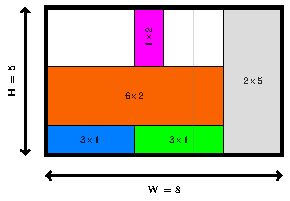
\includegraphics[scale = 1]{Figuras/Exemplo-modelo-altura.pdf}}
            \subfloat[Minimizar perímetro]{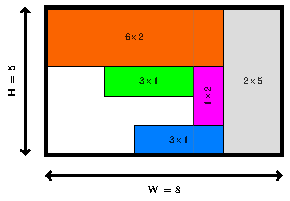
\includegraphics[scale = 1]{Figuras/Exemplo-modelo-perimetro.pdf}}
            \subfloat[Minimizar área]{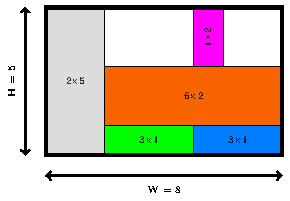
\includegraphics[scale = 1]{Figuras/Exemplo-modelo-area.pdf}}
            % \includegraphics{Figuras/nome.pdf}
            \caption{Exemplo de resolução do problema com três abordagens que desconsideram a rotação dos itens.}
            \label{Fig-Exemplos-sem-rotacao}
        \end{figure}
    
    
        Considerar a rotação dos itens em cada abordagem abre possibilidade para que novas configurações ótimas, que solucionem o problema, possam ser encontradas. Na Figura~\ref{Fig-Exemplos-com-rotacao} são exibidos o resultado dos mesmos modelos considerando a rotação dos itens. Nesse exemplo, os resultados mostram que ainda era possível otimizar a área aproveitada do objeto rotacionando alguns itens. Comparado ao primeiro exemplo, as soluções obtidas por esses métodos com a rotação dos itens demonstram ser ainda melhores: o modelo da altura conseguiu reduzir os espaços vagos e os modelos do perímetro e da área conseguiram entregar uma solução ótima com o máximo aproveitamento da área do objeto.
    
        %%% [FIGURA][EXEMPLO MODELOS COM ROTACAO] %%%%%%%%%%%%%%%%%%%%%%%%%%%%%
        \begin{figure}[htbp]
            \centering
            \subfloat[Minimizar altura]{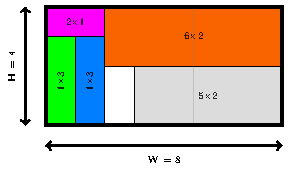
\includegraphics[scale = 1]{Figuras/Exemplo-modelo-altura-rotacao.pdf}}
            \subfloat[Minimizar perímetro]{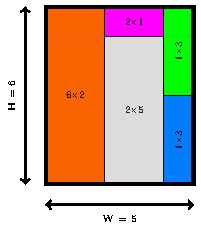
\includegraphics[scale = 1]{Figuras/Exemplo-modelo-perimetro-rotacao.pdf}} \\
            \subfloat[Minimizar área]{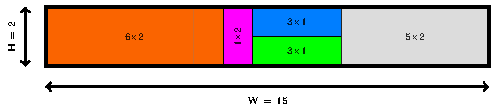
\includegraphics[scale = 1]{Figuras/Exemplo-modelo-area-rotacao.pdf}}
            % \includegraphics{Figuras/nome.pdf}
            \caption{Exemplo de resolução do problema com três abordagens que consideram a rotação dos itens.}
            \label{Fig-Exemplos-com-rotacao}
        \end{figure}
    \end{comment}

    Apesar da simplicidade, o problema de corte e empacotamento bidimensional é classificado como um problema \emph{NP-difícil} (\cite{Garey1990}), (\cite{Lodi2002}). Quanto maior a demanda de itens, mais tempo é necessário para o método aplicado encontrar uma solução. Sendo assim, %a utilização de heurísticas ou de meta-heurísticas, na resolução do problema, pode ser uma vantagem para encontrar melhores resultados no menor intervalo de tempo.
    é necessário buscar meios mais rápidos e eficientes para resolver o problema em menos tempo.

    Para otimizar o tempo de resolução do problema de corte e empacotamento bidimensional com corte não-guilhotinado, desconsiderando a rotação dos itens, é proposto neste projeto institucional de iniciação científica quatro métodos de solução, que consideram as dimensões do objeto (largura e altura) como abertas. Com isso, alguns testes serão realizados com instâncias presentes na literatura para analisar o desempenho do modelo exato formulado e comprovar se as abordagens apresentadas são realmente eficientes na resolução do problema.